\documentclass[letter]{book}

%%%%%% Import Package %%%%%%
\usepackage{graphicx}
\usepackage[unicode]{hyperref}
\usepackage{cite}
\usepackage{indentfirst}
\usepackage{multirow}
\usepackage{indentfirst}
\usepackage{titlesec}
\usepackage{xcolor}
\usepackage{listings}
\usepackage{fontspec,xunicode,xltxtra}
\usepackage{xeCJK}
\usepackage{hyperref}
\usepackage{enumerate}
\usepackage{epigraph}
\usepackage{amsmath}
\usepackage[xindy]{glossaries}
\usepackage{fancyhdr}
\usepackage{amsmath}
%\usepackage{TikZ}
\usepackage{ifthen}
\usepackage{longtable}

%%%% 下面的命令设置行间距与段落间距 %%%%
\linespread{1.4}
% \setlength{\parskip}{1ex}
\setlength{\parskip}{0.5\baselineskip}

%Set Code Format%
\lstloadlanguages{C, csh, make,python,Java}
\lstset{	  
	alsolanguage= XML,  
	tabsize=4, %  
	frame=shadowbox, %把代码用带有阴影的框圈起来  
	commentstyle=\color{red!50!green!50!blue!50},%浅灰色的注释  
	rulesepcolor=\color{red!20!green!20!blue!20},%代码块边框为淡青色  
	keywordstyle=\color{blue!90}\bfseries, %代码关键字的颜色为蓝色,粗体  
	showstringspaces=false,%不显示代码字符串中间的空格标记  
	stringstyle=\ttfamily, % 代码字符串的特殊格式  
	keepspaces=true, %  
	breakindent=22pt, %  
	numbers=left,%左侧显示行号 往左靠,还可以为right,或none,即不加行号  
	stepnumber=1,%若设置为2,则显示行号为1,3,5,即stepnumber为公差,默认stepnumber=1  
	%numberstyle=\tiny, %行号字体用小号  
	numberstyle={\color[RGB]{0,192,192}\tiny} ,%设置行号的大小,大小有tiny,scriptsize,footnotesize,small,normalsize,large等  
	numbersep=8pt,  %设置行号与代码的距离,默认是5pt  
	basicstyle=\footnotesize, % 这句设置代码的大小  
	showspaces=false, % 
	escapechar=`,
	flexiblecolumns=true, %  
	breaklines=true, %对过长的代码自动换行  
	breakautoindent=true,%  
	breakindent=4em, %  	   
	aboveskip=1em, %代码块边框  
	tabsize=4,  
	showstringspaces=false, %不显示字符串中的空格  
	backgroundcolor=\color[RGB]{245,245,244},   %代码背景色  
	%backgroundcolor=\color[rgb]{0.91,0.91,0.91}    %添加背景色  
	escapeinside={``}{\_},  %在``里显示中文  
	%% added by http://bbs.ctex.org/viewthread.php?tid=53451  
	fontadjust,  
	captionpos=t,  
	framextopmargin=2pt,framexbottommargin=2pt,abovecaptionskip=-3pt,belowcaptionskip=3pt,  
	xleftmargin=4em,xrightmargin=4em, % 设定listing左右的空白  
	texcl=true
}

\graphicspath{{./Image/common/}{./Image/Api/}{./Image/InterfaceDesign/}{./Image/Attachment/}}

\begin{document}


\begin{titlepage}

\begin{center}


% Upper part of the page

\includegraphics[width=0.15\textwidth]{./logo}\\[1cm]    

\textsc{\LARGE University of Beer}\\[1.5cm]

\textsc{\Large Final year project}\\[0.5cm]


% Title
%\rule{3mm}{.1pt}
\hrule[1.5cm]


\hrule[1mm]{5mm}%


{ \huge \bfseries Lager brewing techniques}\\[0.4cm]

%\HRule \\[1.5cm]

% Author and supervisor
\begin{minipage}{0.4\textwidth}
\begin{flushleft} \large
\emph{Author:}\\
John \textsc{Smith}
\end{flushleft}
\end{minipage}
\begin{minipage}{0.4\textwidth}
\begin{flushright} \large
\emph{Supervisor:} \\
Dr.~Mark \textsc{Brown}
\end{flushright}
\end{minipage}

\vfill

% Bottom of the page
{\large \today}

\end{center}

\end{titlepage}

\part{Framework}

\section*{Spring}

\subsection{Spring Boot开发者工具}

在build.gradle文件里添加开发工具:

\begin{lstlisting}[language=Bash]
compile "org.springframework.boot:spring-boot-devtools"
\end{lstlisting}

在激活了开发者工具后,Classpath里对文件做任何修改都会触发应用程序重启。为了让重启速度够快,不会修改的类(比如第三方JAR文件里的类)都加载到了基础类加载器里,而应用程序的代码则会加载到一个单独的重启类加载器里。检测到变更时,只有重启类加载器重启。

\subsection*{JDBC数据库重连}

在数据库重启后,程序无法重新连接到数据库。程序使用的是Hikari,找到了如下属性:

\begin{lstlisting}[language=Bash]
# 使用Hikari pool时,是否允许连接池暂停,默认为: false
spring.datasource.allow-pool-suspension=true
\end{lstlisting}

可以将连接池到c3p0,c3p0连接池本身具有数据库重连机制。目前常见到连接池如下表所示:

\begin{tabular}{|c|c|c|p{8cm}|c|}
	\hline
	\multirow{1}{*}{序号}
	& \multicolumn{1}{c|}{名称}  
	& \multicolumn{1}{c|}{协议} 
	& \multicolumn{1}{c|}{备注}\\			
	\cline{1-4}
	1 & c3p0 &  LGPL v.2.1  & C3P0是一个开源数据连接池,Hibernate3.0默认自带的数据连接池,性能比较稳定。\\
	\hline
	2 & HikariCP & Apache 2.0 & Fast, simple, reliable. HikariCP is a "zero-overhead" production ready JDBC connection pool. At roughly 130Kb, the library is very light. \\
	\hline
	3 & Druid & Apache 2.0 & Druid是Java语言中最好的数据库连接池。Druid能够提供强大的监控和扩展功能。 \\
	\hline
	4 & DBCP & Apache 2.0 & DBCP(DataBase connection pool),是 apache 上的一个 java 连接池项目,也是 tomcat 使用的连接池组件。单独使用dbcp需要2个包:commons-dbcp.jar,commons-pool.jar \\
	\hline
	5 & BoneCP & Apache 2.0 & 使用HikariCP替代\\
	\hline
\end{tabular}

登陆服务器,使用命令查看正常的数据库连接:

\begin{lstlisting}[language=Bash]
lsof -i:5236
\end{lstlisting}

输出的结果如下:

\begin{lstlisting}
COMMAND   PID USER   FD   TYPE  DEVICE SIZE/OFF NODE NAME
java    20026   hl   38u  IPv4 2197171      0t0  TCP localhost:58220->localhost:padl2sim (ESTABLISHED)
java    20026   hl   42u  IPv4 2197527      0t0  TCP localhost:58222->localhost:padl2sim (ESTABLISHED)
java    20026   hl   43u  IPv4 2197176      0t0  TCP localhost:58224->localhost:padl2sim (ESTABLISHED)
java    20026   hl   44u  IPv4 2197177      0t0  TCP localhost:58226->localhost:padl2sim (ESTABLISHED)
java    20026   hl   45u  IPv4 2197178      0t0  TCP localhost:58228->localhost:padl2sim (ESTABLISHED)
java    20026   hl   46u  IPv4 2197179      0t0  TCP localhost:58230->localhost:padl2sim (ESTABLISHED)
java    20026   hl   47u  IPv4 2197180      0t0  TCP localhost:58232->localhost:padl2sim (ESTABLISHED)
java    20026   hl   48u  IPv4 2197181      0t0  TCP localhost:58234->localhost:padl2sim (ESTABLISHED)
java    20026   hl   49u  IPv4 2197182      0t0  TCP localhost:58236->localhost:padl2sim (ESTABLISHED)
java    20026   hl   50u  IPv4 2197536      0t0  TCP localhost:58238->localhost:padl2sim (ESTABLISHED)
\end{lstlisting}

在程序启动时,并没有真正建立TCP连接。只有真正的接受到请求查询数据库时,程序才与数据库建立TCP连接。此处建立了10个TCP连接。而Hikari默认的最大连接池数量也为10个。如下配置设启连接池连接池时,初始建立的连接数量为5个:

\begin{lstlisting}
spring.datasource.initial-size=5
\end{lstlisting}

在Spring中配置数据源类型如下:

\begin{lstlisting}
# 指定数据源类型
spring.datasource.type=com.zaxxer.hikari.HikariDataSource
\end{lstlisting}

Hikari默认的数据源默认的连接池数量为10个,默认的数量在HikariConfig类中进行的设置。为什么修改Spring的Initial Size数量会影响Hikari的连接数量呢?如果不配置数据源,Spring Boot默认的数据源是:

\begin{lstlisting}
org.apache.tomcat.jdbc.pool.DataSource
\end{lstlisting}

但是在实际开发中,可能需要使用自己是熟悉的数据源或者其他性能比较高的数据源。此时就可以通过制定Spring的数据源类型来实现。

停止数据库:

\begin{lstlisting}[language=Bash]
nohup sudo /opt/dmdbms/bin/dmserver /opt/dmdbms/data/DAMENG/dm.ini -noconsole &
\end{lstlisting}

在反复研究后发现,程序并未使用HikariCP连接池,而是使用的Spring JDBC连接池,所以在初始化Datasource时指定连接池,如下代码片段所示:

\begin{lstlisting}[language=Java]
@Configuration
@Data
@ConfigurationProperties(prefix = "spring.datasource")
public class DataSourceConfig {

	private String jdbcUrl;
	
	private String username;
	
	private String driverClassName;
	
	private String password;
	
	@Bean
	@Primary
	public DataSource primaryDataSource() {
		HikariConfig hikariConfig = new HikariConfig();
		hikariConfig.setDriverClassName(driverClassName);
		hikariConfig.setJdbcUrl(jdbcUrl);
		hikariConfig.setUsername(username);
		hikariConfig.setPassword(password);
		hikariConfig.setMaximumPoolSize(5);
		hikariConfig.setConnectionTestQuery("SELECT 1");
		hikariConfig.setPoolName("springHikariCP");
		hikariConfig.addDataSourceProperty("dataSource.cachePrepStmts", "true");
		hikariConfig.addDataSourceProperty("dataSource.prepStmtCacheSize", "250");
		hikariConfig.addDataSourceProperty("dataSource.prepStmtCacheSqlLimit", "2048");
		hikariConfig.addDataSourceProperty("dataSource.useServerPrepStmts", "true");
		HikariDataSource dataSource = new HikariDataSource(hikariConfig);
		return dataSource;
	}
}
\end{lstlisting}

\subsection{读取properties属性}

\subsubsection{读取自定义属性}

有时需要读取自定义属性,以配置HikariCP连接池为例,在application.properties文件指定指定配置:

\begin{lstlisting}
spring.datasource.hikari.jdbc-url=jdbc:dm://dn4:5236/DMSERVER
\end{lstlisting}

在类中获取配置相应的值,注意需要添加Data注解,否则需要手写get和set方法:

\begin{lstlisting}[language=Java]
@Configuration
@Data
@ConfigurationProperties(prefix = "spring.datasource.hikari")
public class DataSourceConfig {
	private String jdbcUrl;
}
\end{lstlisting}

由于此处注解是默认写在application.properties配置文件中,所以在ConfigurationProperties中可以不指定路径。否则需要使用locations指定配置文件路径。

\subsection{jps}

jps(Java Virtual Machine Process Status Tool)是JDK 1.5提供的一个显示当前所有java进程pid的命令。jdk中的jps命令可以显示当前运行的java进程以及相关参数,它的实现机制如下:

java程序在启动以后,会在java.io.tmpdir指定的目录下,就是临时文件夹里,生成一个类似于hsperfdata\_User的文件夹,这个文件夹里(在Linux中为/tmp/hsperfdata\_\{userName\}/),有几个文件,名字就是java进程的pid,因此列出当前运行的java进程,只是把这个目录里的文件名列一下而已。 至于系统的参数什么,就可以解析这几个文件获得。hsperfdata的含义就是HotSpot Performance Data。

\begin{lstlisting}[language=Bash]
nohup java -jar -Xmx2g credit-system-web-boot-1.0.0.jar --spring.config.location=application-jenkins.properties &
\end{lstlisting}


\newpage
\section*{Groovy}

\section{Python}

Python是FLOSS(自由/开放源码软件)之一。你可以自由地发布这个软件的拷贝、阅读它的源代码、对它做改动、把它的一部分用于新的自由软件中。Python希望看到一个更加优秀的人创造并经常改进。由于它的开源本质,Python已经被移植在许多平台上(经过改动使它能够工作在不同平台上)。如果你小心地避免使用依赖于系统的特性,那么你的所有Python程序无需修改就可以在下述任何平台上面运行。这些平台包括Linux、Windows、FreeBSD、Macintosh、Solaris、OS/2、Amiga、AROS、AS/400、BeOS、OS/390、z/OS、Palm OS、QNX、VMS、Psion、Acom RISC OS、VxWorks、PlayStation、Sharp Zaurus、Windows CE甚至还有PocketPC、Symbian以及Google基于linux开发的Android平台!

\subsection{基础}

查看Python已经安装了哪些模块,可以直接在Python环境中输入help('modules')命令。在Pycharm中设置Python路径在Preference->Project Interpreter中。

\begin{lstlisting}[language=Bash]
# 安装MySQL
sudo apt-get install mysql-server -y
# 安装pip
sudo apt-get install python-pip python-dev build-essential
# 安装MySQL驱动
sudo pip install mysql-python
<<<<<<< HEAD
# 安装beautifulsoup4
sudo pip install beautifulsoup4
=======
# 安装Beautiful Soup
sudo pip install beautifulsoup4
# openpyxl来处理xml文件
sudo pip install openpyxl
>>>>>>> 4e1bb2f54143f9979a2dcb5a27193e327bd09a9a
\end{lstlisting}

\subsection{Beautiful Soup}

Beautiful Soup 是用Python写的一个HTML/XML的解析器,它可以很好的处理不规范标记并生成剖析树(parse tree)。 它提供简单又常用的导航(navigating),搜索以及修改剖析树的操作。Beautiful Soup提供一些简单的、python式的函数用来处理导航、搜索、修改分析树等功能。它是一个工具箱,通过解析文档为用户提供需要抓取的数据,因为简单,所以不需要多少代码就可以写出一个完整的应用程序。如下代码片段展示爬取豆瓣书籍详情页的书籍信息:

\begin{lstlisting}[language=Bash]
def get_single_book_detail_info(url):
	try:
		req = urllib2.Request(url, headers=hds[np.random.randint(0, len(hds))])
		source_code = urllib2.urlopen(req).read()
		plain_text = str(source_code)
	except (urllib2.HTTPError, urllib2.URLError), e:
		print e
	soup = BeautifulSoup(plain_text)
	list_soup = soup.find('div', {'id': 'info'}).findAll('span')
	return list_soup
\end{lstlisting}

find方法直接返回结果,findAll方法返回符合条件的结果。

\subsection{爬取豆瓣书籍}

向数据库中保存数据:

\begin{lstlisting}[language=Python]
def save_to_mysql():
	try:
		conn = MySQLdb.connect(host='localhost', user='root', passwd='123456', port=3306)
		cur = conn.cursor()
		conn.select_db('dolphin')
		value = ['hi rollen']
		cur.execute('insert into book(name) values(%s)', value)
		conn.commit()
		cur.close()
		conn.close()
	
	except MySQLdb.Error, e:
		print "Mysql Error %d: %s" % (e.args[0], e.args[1])
\end{lstlisting}

在根据标签爬取的书籍列表中,信息不够全面,比如ISBN号码就没有。所以需要爬到每本书籍的详情页面。

\subsection{抓取技巧}

\paragraph{防止IP被封}在爬取豆瓣的页面时,如果一分钟请求超过一定次数(一说40次),豆瓣会将请求的IP加入黑名单。所以一是爬取的频率不要太高,而是可以使用代理来爬取。服务端对IP访问对阈值也有限制,因为按照正常情况下,一个用户不会大批量对请求一个网站的,所以超过了规定的请求次数也会触发封锁。还可以让请求不那么有规律,让服务器无法通过请求的频率判断是机器还是人类,一般人类访问请求的频率是不固定的。

\paragraph{模仿浏览器}有些网站会检查你是不是真的浏览器访问,还是机器自动访问的。这种情况,加上User-Agent,表明你是浏览器访问即可。有时还会检查是否带Referer信息还会检查你的Referer是否合法,一般再加上Referer。在此次抓取的过程中,模仿浏览器:

\begin{lstlisting}[language=Python]
# Some User Agents
headers = [{'User-Agent': 'Mozilla/5.0 (Windows; U; Windows NT 6.1; en-US; rv:1.9.1.6) Gecko/20091201 Firefox/3.5.6'}, \
{
'User-Agent': 'Mozilla/5.0 (Windows NT 6.2) AppleWebKit/535.11 (KHTML, like Gecko) Chrome/17.0.963.12 Safari/535.11'}, \
{'User-Agent': 'Mozilla/5.0 (compatible; MSIE 10.0; Windows NT 6.2; Trident/6.0)'}]
\end{lstlisting}

在HTTP请求头中,添加浏览器相关标识,让服务器认定为来自浏览器的请求。

\paragraph{避免重复抓取}

\paragraph{海量数据}

\subsection{sh: mysql\_config: command not found解决办法}

首先需要安装MySQL,安装完成后,打开终端,输入下方语句修改环境变量:

\begin{lstlisting}[language=Bash]
# 安装python-devel
sudo dnf install python-devel -y
# 解决fatal error: Python.h: No such file or directory
sudo dnf install python-devel --allowerasing
PATH="$PATH":/usr/local/mysql/bin
\end{lstlisting}

设置完成之后,输入如下语句安装MySQL Python:

\begin{lstlisting}[language=Bash]
sudo pip install mysql-python
\end{lstlisting}

\section{React}

\subsection{Cookie}

The browser is expected to support 20 cookies for each Web server, 300 cookies total, and may limit cookie size to 4 KB each.在Chrome中查看Cookie可以直接在Console中输入:

\begin{lstlisting}[language=Bash]
document.cookie
\end{lstlisting}

服务器端像客户端发送Cookie是通过HTTP响应报文实现的,在Set-Cookie中设置需要像客户端发送的cookie,cookie格式如下:

\begin{lstlisting}
Set-Cookie: “name=value;domain=.domain.com;path=/;expires=Sat, 11 Jun 2016 11:29:42 GMT;HttpOnly;secure”
\end{lstlisting}

其中name=value是必选项,其它都是可选项。如果在Cookie中设置了"HttpOnly"属性,那么通过程序(JS脚本、Applet等)将无法读取到Cookie信息,这样能有效的防止XSS攻击。当secure设置为true时,表示创建的 Cookie 会被以安全的形式向服务器传输,也就是只能在 HTTPS 连接中被浏览器传递到服务器端进行会话验证,如果是 HTTP 连接则不会传递该信息,所以不会被盗取到Cookie 的具体内容。Cookie的主要构成如下:

\begin{lstlisting}
name:一个唯一确定的cookie名称。通常来讲cookie的名称是不区分大小写的。
value:存储在cookie中的字符串值。最好为cookie的name和value进行url编码
domain:cookie对于哪个域是有效的。所有向该域发送的请求中都会包含这个cookie信息。这个值可以包含子域(如:yq.aliyun.com),也可以不包含它(如:.aliyun.com,则对于aliyun.com的所有子域都有效).
path: 表示这个cookie影响到的路径,浏览器跟会根据这项配置,像指定域中匹配的路径发送cookie。
expires:失效时间,表示cookie何时应该被删除的时间戳(也就是,何时应该停止向服务器发送这个cookie)。如果不设置这个时间戳,浏览器会在页面关闭时即将删除所有cookie;不过也可以自己设置删除时间。这个值是GMT时间格式,如果客户端和服务器端时间不一致,使用expires就会存在偏差。
max-age: 与expires作用相同,用来告诉浏览器此cookie多久过期(单位是秒),而不是一个固定的时间点。正常情况下,max-age的优先级高于expires。
HttpOnly: 告知浏览器不允许通过脚本document.cookie去更改这个值,同样这个值在document.cookie中也不可见。但在http请求张仍然会携带这个cookie。注意这个值虽然在脚本中不可获取,但仍然在浏览器安装目录中以文件形式存在。这项设置通常在服务器端设置。
secure: 安全标志,指定后,只有在使用SSL链接时候才能发送到服务器,如果是http链接则不会传递该信息。就算设置了secure 属性也并不代表他人不能看到你机器本地保存的 cookie 信息,所以不要把重要信息放cookie就对了
\end{lstlisting}

\paragraph{Max Age}查看Cookie类的setMaxAge(int expiry)方法说明:这个类用于给Cookie设置最大的年龄,以秒为单位。expiry - an integer specifying the maximum age of the cookie in seconds; if negative, means the cookie is not stored; if zero, deletes the cookie.如果这个方法的参数给的是正值,表明cookie在超过指定的年龄时间后会消亡。负值意味着cookie不是永久性存储的,在浏览器关闭的时候将会被删除。这个方法的参数如果是零值将会导致cookie被删除。Expire指定了cookie的生存期,默认情况下cookie是暂时存在的,他们存储的值只在浏览器会话期间存在,当用户推出浏览器后这些值也会丢失,如果想让cookie存在一段时间,就要为expires属性设置为未来的一个过期日期。现在已经被max-age属性所取代,max-age用秒来设置cookie的生存期。

\part{OS}

\section{Linux}

在使用apt-get时,有时可能会遇到依赖损坏的情况,那么可以执行如下命令,尝试修复依赖:

\begin{lstlisting}[language=Bash]
sudo apt-get -f install 
\end{lstlisting}

f参数表示尝试修正系统依赖损坏处。

\subsection{shell}

\paragraph{读取配置文件}在编写自动化部署脚本的时候需要读取配置文件version.properties中的版本号,直接使用source命令即可:

\begin{lstlisting}[language=Bash]
# version.properties文件中直接写VERSION\_CODE=1.0.2即可
source /Users/dolphin/source/credit-system/gradle/version.properties
# 输出1.0.2
echo $VERSION_CODE
\end{lstlisting}

在Gradle中也可以直接读取version.properties中的内容,这样编译打包发布就可以通过脚本自动化完成。

\paragraph{文件是否存在}

Shell下判斷文件是否存在:

\begin{lstlisting}[language=Bash]
myFile="/opt/app/backend/app.pid"

if [ -f "$myFile" ]; then
	kill `cat /opt/app/backend/app.pid`
fi
\end{lstlisting}

\paragraph{大小写不敏感}

有时文件前缀是大写字母,在使用Tab按键自动提示时就必须首先输入大写字母匹配才有效果,总体来说不是非常方便。所以可以设置shell大小写不敏感,就不需要再重复做一次大小写转换操作了:

\begin{lstlisting}[language=Bash]
echo "set completion-ignore-case on">>~/.inputrc
\end{lstlisting}

设置完毕后重新打开终端即可。

\subsection{自动部署}

\begin{lstlisting}[language=Bash]
#!/usr/bin/env bash

#
# 一键部署后端项目到远程1台或多台服务器
# 发布流程为:编译构建-打包-发布包-拷贝包到指定目录-解压包
# 注:本机需要安装Ansible并与服务器做免密登录
#
# 2017-05-25 dolphin 增加动态读取版本号,根据版本自动发布程序
#

# 当使用未初始化的变量时,程序自动退出
set -u

# 当任何一行命令执行失败时,自动退出脚本
set -e

# send=`date '+%Y-%m-%d %H:%M:%S'`
CURRENT\_TIME=`date '+%Y%m%d%H%M%S'`

echo "$CURRENT_TIME"

PROGRAM_PATH_INFORMATION_CENTER="/opt/app/backend"
SERVER_IP="192.168.1.101"
LOGIN_USER="root"
LOCAL_PATH="./cc-web-boot/build/libs"

# Read program version number
source version.properties
echo "$VERSION"

PROGRAM_NAME="credit-system-web-boot-$VERSION.jar"
echo "$PROGRAM_NAME"

echo "开始构建..."
# Build project
./gradlew -p cc-web-boot -x test build
./gradlew -p cc-etl-sechedule -x test build

echo "开始拷贝..."
# publish project
scp $LOCAL_PATH/$PROGRAM_NAME $LOGIN_USER@$SERVER_IP:~/app-soft/
scp start.sh $LOGIN_USER@$SERVER_IP:$PROGRAM_PATH_INFORMATION_CENTER
scp version.properies $LOGIN_USER@$SERVER_IP:$PROGRAM_PATH_INFORMATION_CENTER

ansible webservers -m command -a "date"

echo "停止站点..."
ansible webservers -m command -a "chdir=$PROGRAM_PATH_INFORMATION_CENTER bash ./stop.sh"

echo "等待站点停止..."
sleep 10

echo "备份站点..."
# 备份当前站点
ansible webservers -m command -a "mv $PROGRAM_PATH_INFORMATION_CENTER/$PROGRAM_NAME $PROGRAM_PATH_INFORMATION_CENTER/$PROGRAM_NAME-$CURRENT_TIME"

echo "拷贝新文件..."
ansible webservers -a "mv ~/app-soft/$PROGRAM_NAME $PROGRAM_PATH_INFORMATION_CENTER"

echo "启动站点..."
ansible webservers -m shell -a "bash ./start.sh chdir=$PROGRAM_PATH_INFORMATION_CENTER"

echo "部署完成"
\end{lstlisting}

\subsection{环境变量}

Linux 分 shell变量(set),用户变量(env), shell变量包含用户变量,export是一种命令工具,是显示那些通过export命令把shell变量中包含的用户变量导入给用户变量的那些变量.删除Linux环境变量:

\begin{lstlisting}[language=Bash]
# 查看环境变量
echo $http_proxy
env
# 删除环境变量
unset http_proxy
\end{lstlisting}

set命令显示(设置)shell变量 包括的私有变量以及用户变量,不同类的shell有不同的私有变量 bash,ksh,csh每中shell私有变量都不一样。env命令显示(设置)用户变量变量。export命令显示(设置)当前导出成用户变量的shell变量。

\begin{tabular}{cp{8cm}c}
	\hline
	\multirow{1}{*}{序号}
	& \multicolumn{1}{c}{名称}  \\
	\hline			
	/etc/profile  & 此文件为系统的每个用户设置环境信息,当用户第一次登录时,该文件被执行.并从/etc/profile.d目录的配置文件中搜集shell的设置 \\	
	/etc/environment & 在登录时操作系统使用的第二个文件,系统在读取你自己的profile前,设置环境文件的环境变量 \\
	/etc/bashrc & 为每一个运行bash shell的用户执行此文件.当bash shell被打开时,该文件被读取\\
	~/.profile & 每个用户都可使用该文件输入专用于自己使用的shell信息,当用户登录时,该文件仅仅执行一次!默认情况下,它设置一些环境变量,执行用户的.bashrc文件\\
	~/.bashrc &  该文件包含专用于你的bash shell的bash信息,当登录时以及每次打开新的shell时,该文件被读取\\
	\hline
\end{tabular}

有时在Bash记录历史命令时,需要忽略掉重复的命令等。可以做如下设置:

\begin{lstlisting}[language=Bash]
# 忽略[连续]重复命令
HISTCONTROL=ignoredups
# 清除重复命令
# HISTCONTROL=erasedups
# 忽略特定命令
HISTIGNORE="[   ]*:ls:ll:cd:vi:pwd:sync:exit:history*"
# 命令历史文件大小10M
HISTFILESIZE=1000000000
# 保存历史命令条数10W
HISTSIZE=1000000
\end{lstlisting}

以上配置可以通过 set | grep HIST 查看可选项.当打开多个终端,关闭其中一个终端时,会覆盖其他终端的命令历史, 这里我们采用追加的方式避免命令历史文件 .bash\_history 文件被覆盖。 再次打开 ~/.bashrc 文件添加下面这一句.

\begin{lstlisting}[language=Bash]
shopt -s histappend
\end{lstlisting}

更多 shopt 可选项可以通过 echo \$SHELLOPTS 命令查看。



\subsubsection{screen}

GNU Screen是一款由GNU计划开发的用于命令行终端切换的自由软件。用户可以通过该软件同时连接多个本地或远程的命令行会话,并在其间自由切换。在使用nohup时,有一个缺点就是交互性很低,例如后台启动OpenVPN时,需要输入预先设置的认证密码。但是使用nohup命令启动时,无法显示密码输入入口。此时就需要使用screen命令了。输入如下的命令:

\begin{lstlisting}[language=Bash]
screen sudo openvpn client.conf
\end{lstlisting}

接着在跳出的窗口中,输入密码。按下Ctrl + A后再按下d键,暂时断开screen会话即可。只要Screen本身没有终止,在其内部运行的会话都可以恢复。这一点对于远程登录的用户特别有用——即使网络连接中断,用户也不会失去对已经打开的命令行会话的控制。只要再次登录到主机上执行screen -r就可以恢复会话的运行。同样在暂时离开的时候,也可以执行分离命令detach,在保证里面的程序正常运行的情况下让Screen挂起(切换到后台)。这一点和图形界面下的VNC很相似。查看当前系统中有哪些screen会话:

\begin{lstlisting}[language=Bash]
screen -ls
\end{lstlisting}

该命令会列出当前系统中所有的screen会话,重新打开会话:

\begin{lstlisting}[language=Bash]
screen -r 12865
\end{lstlisting}

正常情况下,当你退出一个窗口中最后一个程序(通常是bash)后,这个窗口就关闭了。另一个关闭窗口的方法是使用C-a k,这个快捷键杀死当前的窗口,同时也将杀死这个窗口中正在运行的进程。如果一个Screen会话中最后一个窗口被关闭了,那么整个Screen会话也就退出了,screen进程会被终止。除了依次退出/杀死当前Screen会话中所有窗口这种方法之外,还可以使用快捷键C-a :,然后输入quit命令退出Screen会话。需要注意的是,这样退出会杀死所有窗口并退出其中运行的所有程序。其实C-a :这个快捷键允许用户直接输入的命令有很多,包括分屏可以输入split等,这也是实现Screen功能的一个途径

\subsubsection{查看Linux信息}

\begin{lstlisting}[language=Bash]
# Linux查看版本当前操作系统内核信息
uname -a 
\end{lstlisting}

\subsection{XFCE桌面}

占用资源较GNOME ,KDE较少。适合老机器,轻量级桌面。与windows界面环境类似。许多不习惯GNOME 3 ,Unity新桌面的同学,很多选择了XFCE 4.8,包括Linus大神同学。

\subsection{Fedora访问共享文件夹}

在局域网里,有时需要使用Fedora 24访问Windows共享文件夹。在Fedora中输入命令:

\begin{lstlisting}[language=Bash]
sudo mount -t cifs -o username="aaa",uid="dolphin",gid="dolphin" //10.55.10.2/data /home/dolphin/software
\end{lstlisting}

一般提示权限错误是由于用户名密码输入错误。aaa为Windows机器的用户名,uid为当前Fedora账户的名称,gid为当前Fedora用户组的名称。10.55.10.2为Windows账户的IP,data为共享文件夹的名称,与盘符无关。/home/dolphin/software本地Fedora机器的目录。cifs为通用网络文件系统,The Common Internet File System (CIFS) is the standard way that computer users share files across corporate intranets and the Internet. An enhanced version of the Microsoft open, cross-platform Server Message Block (SMB) protocol, CIFS is a native file-sharing protocol in Windows 2000.


\subsection{软件包管理}

根据软件包的名称模糊匹配,查看系统已经安装了哪些软件包:

\begin{lstlisting}[language=Bash]
dpkg -l|grep pcre
yum list installed|grep openssl
# 查看openssl版本
openssl version -a
# yum查看已经安装的软件包
yum list installed
\end{lstlisting}

\subsection{输入法(Input Method)}

有时在Fedora 24中,突然中文输入法切换后无法输入中文了。可以到系统区域和语言(Region\&Language)设置界面,重新删除后再添加即可修复,如图\ref{fig:regionandlanguagesetting}所示。

\begin{figure}[htbp]
	\centering
	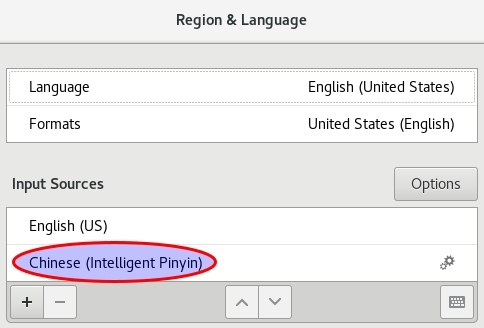
\includegraphics[scale=0.6]{regionandlanguagesetting.jpg}
	\caption{Fedora区域和语言设置}
	\label{fig:regionandlanguagesetting}
\end{figure}

在使用Ubuntu 16.04的搜狗拼音时,有时也会出现各种问题。可以尝试的解决方案包括,登录系统再次重新登入。删除输入法配置后,重新添加输入法,或者使用Google拼音输入法,输入如下命令进行安装:

\begin{lstlisting}[language=Bash]
sudo apt install fcitx-googlepinyin
\end{lstlisting}

安装好后需要重新登入系统,添加输入法配置时才可以选择Google输入法。

\part{Tool}

\newpage

\section{Intellij Idea}

\subsection{Intellij Idea远程调试}

\subsection{Intellij Idea调试慢}

在使用Intellij Idea时调试Spring Boot项目时,启动时突然变慢了,原来启动10几秒,后来启动莫名其妙需要1分钟左右。经过排查是由于打了过多的断点的缘故,删除断点后,启动立即变快了。所以在项目中不能标记太多断点,调试后立即将断点删除。

\subsection{常用设置}

\paragraph{自动换行}有时候,代码太长,滚动滑块不是非常方便。需要设置代码自动换行。

\section*{Gradle}

\subsection{执行流程}

There is a one-to-one relationship between a Project and a "build.gradle" file. During build initialisation, Gradle assembles a Project object for each project which is to participate in the build, as follows:

Create a Settings instance for the build.
Evaluate the "settings.gradle" script, if present, against the Settings object to configure it.
Use the configured Settings object to create the hierarchy of Project instances.
Finally, evaluate each Project by executing its "build.gradle" file, if present, against the project. The projects are evaluated in breadth-wise order, such that a project is evaluated before its child projects. This order can be overridden by calling evaluationDependsOnChildren() or by adding an explicit evaluation dependency using evaluationDependsOn(String).

\subsection{repositories}

在Gradle构建标本build.gradle里,经常会看到如下脚本:

\begin{lstlisting}[language=Java]
repositories {
	maven {
		url 'http://www.eveoh.nl/files/maven2'
	}
	maven {
		url 'http://repox.gtan.com:8078'
	}
	mavenCentral()
	jcenter()
	maven { url 'http://repo.spring.io/plugins-release' }
}
\end{lstlisting}

总的来说,只有两个标准的Android library文件服务器:Jcenter 和 Maven Central。起初,Android Studio 选择Maven Central作为默认仓库。如果你使用老版本的Android Studio创建一个新项目,mavenCentral()会自动的定义在build.gradle中。但是Maven Central的最大问题是对开发者不够友好。上传library异常困难。上传上去的开发者都是某种程度的极客。同时还因为诸如安全方面的其他原因,Android Studio团队决定把默认的仓库替换成jcenter。正如你看到的,一旦使用最新版本的Android Studio创建一个项目,jcenter()自动被定义,而不是mavenCentral()。mavenCentral()表示依赖是从Central Maven 2 仓库中获取的,库的地址是\url{https://repo1.maven.org/maven2}。jcenter表示依赖是从Bintary’s JCenter Maven 仓库中获取的,仓库的地址是\url{https://jcenter.bintray.com},bintray是一家提供全球企业软件开发包托管的商业公司。

\subsection{属性(Properties)}

\subsubsection{Extra Properties}

extra属性一般用于定义常量,All extra properties\footnote{\url{https://docs.gradle.org/current/javadoc/org/gradle/api/Project.html\#extraproperties}} must be defined through the "ext" namespace. Once an extra property has been defined, it is available directly on the owning object (in the below case the Project, Task, and sub-projects respectively) and can be read and updated. Only the initial declaration that needs to be done via the namespace.

\begin{lstlisting}[language=Java]
buildscript {
	ext {
		springBootVersion = '1.4.5.RELEASE'
		jacksonVersion = '2.8.7'
		springfoxVersion = '2.6.1'
		poiVersion = "3.14"
		aspectjVersion = '1.7.4'
	}
}
\end{lstlisting}

Reading extra properties is done through the "ext" or through the owning object.


ext.isSnapshot = version.endsWith("-SNAPSHOT")
if (isSnapshot) {
	// do snapshot stuff
}

\subsection{同时连接内外网}

在工作中,有时需要同时连接封闭的网络和互联网,开发环境需要依赖封闭的内网,与远程的同事交流需要依赖互联网,而封闭的内网与互联网切换是一大痛点,不仅影响效率,同时也影响心情,宝贵的时间就在这样无意义的开关中白白浪费掉了。制造障碍很容易,清除障碍很艰难。

解决双网卡问题,既能保证内网访问的安全,又能避免频繁切换网卡带来的时间开销,可谓一举两得。一般的计算机有有线网卡,也有无线网卡。一般情况下要么使用有线网卡,要么使用无线网卡,在使用无线时,连接上了有线,因为有线网卡的优先级高,故此时仅有有线能够工作,无线网卡可连接但是无法传送数据。实现双网卡的基本思路是删除默认网关,配置各自的网关即可。

\subsubsection{Mac同时连内网外网}

输入如下命令查看Mac的所有网络连接方式:

\begin{lstlisting}[language=Bash]
networksetup -listallnetworkservices
\end{lstlisting}

输出的结果如下:

\begin{lstlisting}
An asterisk (*) denotes that a network service is disabled.
Apple USB Ethernet Adapter
Wi-Fi
Bluetooth PAN
Thunderbolt Bridge
\end{lstlisting}

可以看出Mac可以通过Wi-Fi联网,也可以通过USB有线联网。给指定的网络连接方式设定DNS服务器代码如下:

\begin{lstlisting}[language=Bash]
sudo networksetup -setdnsservers AirPort 192.168.10.200
\end{lstlisting}

清空DNS缓存代码如下:

\begin{lstlisting}[language=Bash]
dscacheutil –flushcache
\end{lstlisting}

输入如下命令查看MacBook的路由表:

\begin{lstlisting}[language=Bash]
netstat -nr
\end{lstlisting}

\subsubsection{Fedora同时连接内外网}

给有线网卡配置地址信息时,内网网卡不要加默认网关,外网网卡加默认网关,并查看无线网卡分配到的地址信息中是否有默认网关。在这里内网是有线网络,外网是无线网络。使用route命令查看默认路由,输出如图\ref{fig:routetable}所示:

\begin{figure}[htbp]
	\centering
	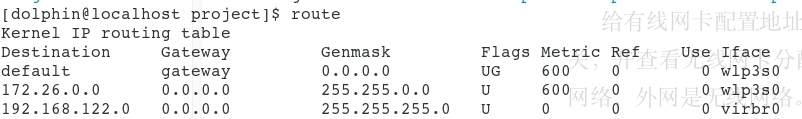
\includegraphics[scale=0.4]{route-table.jpg}
	\caption{查看Kernel路由表}
	\label{fig:routetable}
\end{figure}

其中wlp3s0是无线网卡的名称,此命名规范为v197\footnote{https://www.freedesktop.org/wiki/Software/systemd/PredictableNetworkInterfaceNames/},说明此时的默认路由是无线网卡的路由。metric设置路由跳数,metric值越高,优先级越低。添加-p(permanent)参数永久保存此条路由信息,系统重启后路由也规则也不会丢失。flag的含义如下:

\begin{tabular}{cp{10cm}c}
	\hline
	\multirow{1}{*}{序号}
	& \multicolumn{1}{c}{名称}  \\
	\hline			
	U  & Up表示此路由当前为启动状态 \\	
	H & Host,表示此网关为一主机 \\
	G & Gateway,表示此网关为一路由器\\
	R & Reinstate Route,使用动态路由重新初始化的路由\\
	D & Dynamically,此路由是动态性地写入\\
	M & Modified,此路由是由路由守护程序或导向器动态修改\\
	! & 表示此路由当前为关闭状态\\
	\hline
\end{tabular}

删除默认网关的命令如下:

\begin{lstlisting}[language=Bash]
sudo route del default
\end{lstlisting}

删除一条路由:

\begin{lstlisting}[language=Bash]
sudo route del -net 192.168.122.0 netmask 255.255.255.0
\end{lstlisting}

如果默认路由是外网网关。那么只需要单独为内网设置转发特例,所有59.214.*.*开头的,全部走enp0s26u1u2:

\begin{lstlisting}[language=Bash]
sudo route add -net 59.214.0.0 netmask 255.255.255.0 gw 10.55.10.1 dev enp0s26u1u2
\end{lstlisting}

其中59.214.0.0为内网IP的起始网段,255.255.0.0为内网的子网掩码,内网网关是10.36.40.12,eth0为内网网卡的名称。路由添加最好是添加到开机启动中:

\begin{lstlisting}[language=Bash]
vim /etc/rc.local
\end{lstlisting}

添加删除默认网关:

\begin{lstlisting}[language=Bash]
#添加默认网关
sudo route add default gw 10.55.10.1
#删除默认网关
sudo route del default gw 10.55.10.1
\end{lstlisting}

重启网络服务:

\begin{lstlisting}[language=Bash]
/etc/init.d/networking restart
\end{lstlisting}

此时可以同时访问互联网和局域网中的主机,但是无法访问A网络。访问A网络可通过局域网代理的方式访问,将局域网的一台主机作为代理服务器,本机访问局域网中的代理服务器,代理服务器再将请求转发给A网络。在本机只需要在浏览器中配置好代理服务器即可。以FireFox浏览器为例,在Preference->Advance->Network->Connection->Settings中,增加手动代理配置,地址填写代理主机的地址,端口填写8888,代理服务器运行的是Fiddler。以后,访问内网时就使用FireFox浏览器,访问外网时就使用Google Chrome浏览器。


\subsubsection{Ubuntu同时连接内外网}

\subsubsection{Windows同时连接内外网}


\section{Ansible}

\subsection{Ansible模块}

\paragraph{shell模块}使用shell模块,在远程命令通过/bin/sh来执行;所以,我们在终端输入的各种命令方式,都可以使用; 但是我们自己定义在.bashrc/.bash\_profile中的环境变量shell模块由于没有加载,所以无法识别;如果需要使用自定义的环境变量,就需要在最开始,执行加载自定义脚本的语句;对shell模块的使用可以分成两块:如果待执行的语句少,可以直接写在一句话中:

\begin{lstlisting}[language=bash]
ansible myservers  -a ". .bash_profile;ps -fe |grep sa_q" -m shell
\end{lstlisting}

如果在远程待执行的语句比较多,可写成一个脚本,通过copy模块传到远端,然后再执行;但这样就又涉及到两次ansible调用;对于这种需求,ansible已经为我们考虑到了,script模块就是干这事的;


\section{Nginx}

\subsection{Nginx获取真实IP}

做异地登陆的判断,或者统计ip访问次数等,通常情况下我们使用request.getRemoteAddr()就可以获取到客户端ip,但是当我们使用了nginx作为反向代理后,使用request.getRemoteAddr()获取到的就一直是nginx服务器的ip的地址。Nginx作为HTTP代理转发前端时,后端服务无法获知前端访问客户的IP地址。要获取客户端IP,需要将http\_realip\_module编译进入Nginx中。查看Nginx安装了哪些模块,使用如下命令:

\begin{lstlisting}[language=bash]
nginx -V
\end{lstlisting}

输出结果如下:

\begin{lstlisting}[language=bash]
nginx version: nginx/1.12.0
built by gcc 5.4.0 20160609 (Ubuntu 5.4.0-6ubuntu1~16.04.2) 
built with OpenSSL 1.0.2g-fips  1 Mar 2016 (running with OpenSSL 1.0.2g  1 Mar 2016)
TLS SNI support enabled
configure arguments: --prefix=/etc/nginx --sbin-path=/usr/sbin/nginx --modules-path=/usr/lib/nginx/modules --conf-path=/etc/nginx/nginx.conf --error-log-path=/var/log/nginx/error.log --http-log-path=/var/log/nginx/access.log --pid-path=/var/run/nginx.pid --lock-path=/var/run/nginx.lock --http-client-body-temp-path=/var/cache/nginx/client_temp --http-proxy-temp-path=/var/cache/nginx/proxy_temp --http-fastcgi-temp-path=/var/cache/nginx/fastcgi_temp --http-uwsgi-temp-path=/var/cache/nginx/uwsgi_temp --http-scgi-temp-path=/var/cache/nginx/scgi_temp --user=nginx --group=nginx --with-compat --with-file-aio --with-threads --with-http_addition_module --with-http_auth_request_module --with-http_dav_module --with-http_flv_module --with-http_gunzip_module --with-http_gzip_static_module --with-http_mp4_module --with-http_random_index_module --with-http_realip_module --with-http_secure_link_module --with-http_slice_module --with-http_ssl_module --with-http_stub_status_module --with-http_sub_module --with-http_v2_module --with-mail --with-mail_ssl_module --with-stream --with-stream_realip_module --with-stream_ssl_module --with-stream_ssl_preread_module --with-cc-opt='-g -O2 -fstack-protector-strong -Wformat -Werror=format-security -Wp,-D_FORTIFY_SOURCE=2 -fPIC' --with-ld-opt='-Wl,-Bsymbolic-functions -Wl,-z,relro -Wl,-z,now -Wl,--as-needed -pie'
\end{lstlisting}

此处显示已经编译了http\_realip\_module模块。项目中使用的tengine,经过查看是没有编译http\_realip\_module模块,从tengine官网上下载好源码,输入如下命令进行编译:

\begin{lstlisting}[language=bash]
# 在Ubuntu 14.04 LTS下安装pcre依赖
# pcre:Perl Compatible Regular Expressions
sudo apt-get install libpcre3 libpcre3-dev
# 指定预编译参数,仅仅指定路径
sudo ./configure --prefix=/opt/tengine
# 将realip模块编译进入
sudo ./configure --prefix=/opt/tengine --with-http_realip_module
# 编译
sudo make
# 安装
sudo make install
./configure --prefix=/usr/local/tengine-2.1.2 --with-openssl=/Users/dolphin/source/openssl
\end{lstlisting}

不指定prefix,则可执行文件默认放在/usr /local/bin,库文件默认放在/usr/local/lib,配置文件默认放在/usr/local/etc。其它的资源文件放在/usr /local/share。
你要卸载这个程序,要么在原来的make目录下用一次make uninstall(前提是make文件指定过uninstall),要么去上述目录里面把相关的文件一个个手工删掉。
指定prefix,直接删掉一个文件夹就够了。在编译时,还需要指定pcre的版本,因为Ubuntu 16.04 LTS里有时安装有pcre 3,而部署的电脑上不一定安装有pcre 3,而且pcre 3的源码不容易找到。所以编译命令如下:

\begin{lstlisting}[language=bash]
# 将realip模块编译进入,并指定pcre
sudo ./configure --prefix=/opt/tengine --with-http_realip_module --with-pcre=/root/software/pcre-8.40 --with-openssl=/root/software/openssl-OpenSSL_1_1_0e --without-http_gzip_module

./configure --prefix=/opt/tengine --with-http_realip_module --with-pcre=/root/software/pcre-8.40  --without-http_gzip_module

#本机编译(不成功)
./configure --prefix=/opt/tengine --with-http_realip_module --with-pcre=/home/hldev/Downloads/pcre-8.40 --with-openssl=/home/hldev/Downloads/openssl-OpenSSL_1_0_1e --without-http_gzip_module

#本机编译(成功)
-prefix=/opt/tengine --with-http_realip_module --with-pcre=/home/hldev/Downloads/pcre-8.40 --with-openssl=/home/hldev/software/openssl-OpenSSL_1_0_2g --without-http_gzip_module

# 构建程序
make

#安装程序
make install

#服务器
./configure --prefix=/opt/tengine

./configure: error: SSL modules require the OpenSSL library.
You can either do not enable the modules, or install the OpenSSL library
into the system, or build the OpenSSL library statically from the source
with nginx by using --with-openssl=<path> option.


\end{lstlisting}

其中--with-pcre表示pcre的源代码目录。在编译时,还需要注意openssl的版本,本地电脑版本是1.0.2g,服务端的版本是1.0.1e。服务器端编译Nginx的一个命令:

\begin{lstlisting}[language=bash]
./configure --prefix=/opt/tengine --with-openssl=/usr/local/src/openssl-OpenSSL_1_0_2g/ --without-http_gzip_module --with-pcre=/usr/local/src/pcre-8.40/
\end{lstlisting}

这里编译的时候有一个小细节需要注意,需要将源码包存放到/usr/local/src目录下。一直没有编译成功也许是这个小小的细节,开始时是将源码包随意存放的一个目录。以上编译的命令没有包含Zlib,也没有包含http\_realip\_module模块。最终的编译命令如下:

\begin{lstlisting}[language=bash]
./configure --prefix=/opt/tengine --with-openssl=/usr/local/src/openssl-OpenSSL_1_0_2g/ --without-http_gzip_module --with-pcre=/usr/local/src/pcre-8.40/ --with-zlib=/usr/local/src/zlib-1.2.11 --with-http_realip_module 
\end{lstlisting}

编译完毕之后,输入如下命令:

\begin{lstlisting}[language=bash]
# 查看Tengine版本、模块信息,编译时所使用的参数
./nginx -V
\end{lstlisting}

即可看到http\_realip\_module已经编译到nginx中了。Nginx的http\_realip\_module等于Apache的mod\_rpaf用于接受前端发来的IP head信息,从获取到真是的用户IP。将获取真实IP的模块编译进入Nginx后,还需要在对应的http、server、location中加入以下参数:

\begin{lstlisting}[language=bash]
#指令是告诉nginx,10.10.1.11是我们的反代服务器,不是真实的用户IP
set_real_ip_from 10.10.1.11;
#告诉nginx真正的用户IP是存在X-Forwarded-For请求头中
real_ip_header X-Real-IP;
\end{lstlisting}

其中set\_real\_ip\_from可以指定某个网段。这个指令指定信任的代理IP,它们将会以精确的替换IP转发。0.8.22后可以指定Unix sockets。real\_ip\_header设置需要使用哪个头来确定替换的IP地址。由于项目中使用的Nginx作为反向代理,所以配置如下:

\begin{lstlisting}[language=bash]
location /inapi {
         proxy_pass http://localhost:28080;
         proxy_set_header X-Real-IP $remote_addr;
         proxy_redirect off;
     }
\end{lstlisting}

在另一台电脑上访问服务端,在后端根据新添加的Header获取到的IP地址如图\ref{fig:nginxgetrealip}所示:

\begin{figure}[htbp]
	\centering
	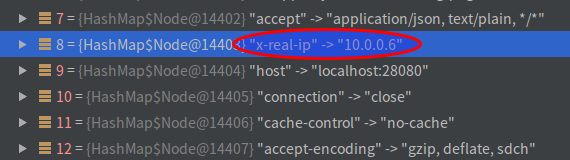
\includegraphics[scale=0.6]{nginxgetrealip.png}
	\caption{Nginx获取用户真实访问IP}
	\label{fig:nginxgetrealip}
\end{figure}

此处获取到的IP是用户的真实IP,而不是反向代理服务器的IP。

\subsection{常见问题}

\paragraph{error while loading shared libraries: libpcre.so.3: cannot open shared object file}

找不到libpcre.so.3文件,在本机搜索了之后,发现文件在目录下:

\begin{lstlisting}[language=bash]
/lib/i386-linux-gnu/libpcre.so.3
/lib/x86_64-linux-gnu/libpcre.so.3
\end{lstlisting}

\paragraph{error while loading shared libraries: libssl.so.1.0.0: cannot open shared object file}

有可能是由于openssl库的位置不对导致的,可以尝试创建软链接解决:

\begin{lstlisting}[language=bash]
ln -s /usr/local/lib64/libssl.so.1.1 /usr/lib64/libssl.so.1.1  
ln -s /usr/local/lib64/libcrypto.so.1.1 /usr/lib64/libcrypto.so.1.1  
\end{lstlisting}

.so 为共享库,是shared object,用于动态连接的,和dll差不多。openssl:多用途的命令行工具,各功能分别使用子命令实现,libcrypto:公共加密库(存放了各种加密算法),libssl:ssl协议的实现。在Ubuntu下可以通过如下命令安装libssl.so.1.0.0:

\begin{lstlisting}[language=bash]
sudo apt-get install libssl1.0.0:amd64
sudo apt-get install libssl1.0.0 libssl-dev

#查看OpenSSL版本
openssl version

#查看系统中对libssl
find / -name libssl.s0*

# 列出openssl包
yum list \*openssl\*
\end{lstlisting}

不过此处不能通过命令安装,只能通过源码编译安装。这里有包: \url{https://pkgs.org/download/libssl1.0.0}。查看当前操作系统支持的openssl:

\begin{lstlisting}[language=bash]
yum --showduplicates list openssl
\end{lstlisting}

寻找包含libssl.so.1.0.0的安装包:

\begin{lstlisting}[language=bash]
yum provides */libssl.so.1.0.0
\end{lstlisting}

在http://rpm.pbone.net/上搜索 openssl1-1.0.0 ,搜到openssl1-1.0.0-4.fc24.x86\_64.rpm。

\url{http://rpmfind.net/linux/rpm2html/search.php?query=openssl&submit=Search+...&system=CentOS&arch=}

\section{Fiddler}

\subsection{Fiddler替换Host}

\section{Charles}

Charles是Mac端的一款截取与分析网络请求的工具,在网络开发中使用其作分析,可以大大提高我们的开发效率。Charles是收费软件,一般可以试用三十天。Charles is an HTTP proxy / HTTP monitor / Reverse Proxy that enables a developer to view all of the HTTP and SSL / HTTPS traffic between their machine and the Internet. This includes requests, responses and the HTTP headers (which contain the cookies and caching information).

\subsection{title}


\section{OpenVPN}

OpenVPN从2001年开始开发,使用的是C语言。此处使用的OpenVPN版本是2.4.1。如果使用Mac下的brew工具安装,则OpenVPN目录在:/usr/local/Cellar/openvpn/2.4.1,OpenVPN的配置文件在:/usr/local/etc/openvpn。目前OpenVPN能在Solaris、Linux、OpenBSD、FreeBSD、NetBSD、Mac OS X与Microsoft Windows以及Android和iOS上运行,并包含了许多安全性的功能。此处的服务器使用的是CentOS 7.3,客户端包含Fedora 24、Ubuntu 14.04、Ubuntu 16.04、Window 7、Windows 10。在OpenVPN网络中查看存活的主机:

\begin{lstlisting}[language=bash]
nmap -A -T4 10.0.0.*
\end{lstlisting}

\subsection{安装}

安装基础包:

\begin{lstlisting}[language=bash]
sudo yum -y install openssl openssl-devel lzo openvpn easy-rsa --allowerasing
#手动安装
wget -c https://swupdate.openvpn.org/community/releases/openvpn-2.4.1.tar.gz
tar -zxvf openvpn-2.4.1.tar.gz
./configure
make && make install
\end{lstlisting}

LZO 是致力于解压速度的一种数据压缩算法,LZO 是 Lempel-Ziv-Oberhumer 的缩写。这个算法是无损算法,参考实现程序是线程安全的。 实现它的一个自由软件工具是lzop。最初的库是用 ANSI C 编写、并且遵从 GNU通用公共许可证发布的。现在 LZO 有用于 Perl、Python 以及 Java 的各种版本。代码版权的所有者是 Markus F. X. J. Oberhumer。

\subsection{生成客户端证书}

生成客户端证书端步骤如下:

\begin{lstlisting}[language=Bash]
#建立一个空的pki结构,生成一系列的文件和目录
./easyrsa init-pki
\end{lstlisting}

PKI:Public Key Infrastructure公钥基础设施。生成请求:

\begin{lstlisting}[language=Bash]
./easyrsa gen-req dolphinfedora
\end{lstlisting}

输入PEM验证码。PEM - Privacy Enhanced Mail,打开看文本格式,以"-----BEGIN..."开头, "-----END..."结尾,内容是BASE64编码。
Apache和*NIX服务器偏向于使用这种编码格式.签约:

\begin{lstlisting}[language=Bash]
#切换到服务端生成rsa的目录
#导入req
./easyrsa import-req ~/client/easyrsa/easy-rsa-master/easyrsa3/pki/reqs/dolphinfedora.req dolphinfedora
#用户签约,根据提示输入服务端的ca密码
./easyrsa sign client dolphinfedora
\end{lstlisting}

PKI:Public Key Infrastructure公钥基础设施。输入PEM验证码。PEM - Privacy Enhanced Mail,打开看文本格式,以"-----BEGIN..."开头, "-----END..."结尾,内容是BASE64编码.查看PEM格式证书的信息:openssl x509 -in certificate.pem -text -noout。Apache和*NIX服务器偏向于使用这种编码格式.服务端生成的文件有:

\begin{tabular}{|c|p{5cm}|c|}
	\hline
	\multirow{1}{*}{文件名称}
	& \multicolumn{1}{c|}{说明(Purpose)} 
	& \multicolumn{1}{c|}{位置} \\			
	\cline{1-3}
	ca.crt  & 根证书(Root CA certificate)件 & Server+All Clients	\\
	\hline
	reqs/server.req  & &\\
	\hline
	reqs/dolphin.req  & &\\
	\hline
	private/ca.key & 根证书私钥(Root CA key) & key signing machine only\\
	\hline
	private/server.key && \\
	\hline
	issued/server.crt & 服务器证书Server Certificate & server only\\
	\hline
	issued/dolphin.crt && \\
	\hline
	dh.pem & Diffie Hellman parameters & server only \\
	\hline
\end{tabular}

客户端生成的文件有:

\begin{tabular}{|c|p{8cm}|c|}
	\hline
	\multirow{1}{*}{序号}
	& \multicolumn{1}{c|}{名称}  \\			
	\cline{1-2}
	private/dolphinclient.key  & \\
	\hline
	reqs/sdolphinclient.req & \\
	\hline
\end{tabular}

拷贝出客户端证书文件:

\begin{lstlisting}[language=Bash]
cp easyrsa/easy-rsa-master/easyrsa3/pki/ca.crt ~/dolphinfedora/
cp easyrsa/easy-rsa-master/easyrsa3/pki/issued/dolphinfedora.crt ~/dolphinfedora/
cp ~/client/easyrsa/easy-rsa-master/easyrsa3/pki/private/dolphinfedora.key ~/dolphinfedora/
\end{lstlisting}


启动OpenVPN:

\begin{lstlisting}[language=Bash]
sudo openvpn server.conf
# Mac下启动OpenVPN
sudo /usr/local/Cellar/openvpn/2.4.1/sbin/openvpn /usr/local/etc/openvpn/client.conf
# 需要以后台交互方式启动时
screen sudo openvpn client.conf
\end{lstlisting}

客户端端配置如下:

\begin{lstlisting}[language=Bash]
client         #指定当前VPN是客户端
dev tun        #必须与服务器端的保持一致
proto udp      #必须与服务器端的保持一致
#指定连接的远程服务器的实际IP地址和端口号
remote 192.168.1.106 1194      
#断线自动重新连接
#在网络不稳定的情况下(例如:笔记本电脑无线网络)非常有用
resolv-retry infinite
nobind         #不绑定特定的本地端口号
persist-key
persist-tun
ca ca.crt      #指定CA证书的文件路径
cert client1.crt       #指定当前客户端的证书文件路径
key client1.key    #指定当前客户端的私钥文件路径
ns-cert-type server      #指定采用服务器校验方式
#如果服务器设置了防御DoS等攻击的ta.key
#则必须每个客户端开启;如果未设置,则注释掉这一行;
tls-auth ta.key 1     
comp-lzo              #与服务器保持一致
#指定日志文件的记录详细级别,可选0-9,等级越高日志内容越详细
verb 3                
\end{lstlisting}

配置ns-cert-type(Netscape Cert Type)指定为server主要是防止中间人攻击(Man-in-the-Middle Attack)。在服务端做如下配置:

\begin{lstlisting}[language=Bash]
nsCertType server
\end{lstlisting}

1.首页总数体现新增数据,总数和本月新入数量
2.综合查询时要体验不同的数据来源,法人和自然人新增一个数据来源字段
3.红黑名单详情中,添加来源字段,要在详情中显示
4.倒出数据自动化功能
5.打印出的界面需要添加来源字段
6.格式固定化,显示固定的字数,后面用省略号代替,鼠标移入时提示全部

\subsection{Mac Book客户端配置}

在Mac下连接OpenVPN需要安装Tunnelblick,Tunnelblick是Mac OS X上的一个OpenVPN的图形化前端界面。Tunnelblick is free software licensed under the GNU General Public License, version 2 and may be distributed only in accordance with the terms of that license.安装好Tunnelblick之后,直接导入相应的设置即可。如下是Mac Book下一个OpenVPN客户端可用配置的示例。

\begin{lstlisting}[language=Bash]
# 定义一个客户端
client
# 和服务器保持一致
dev tun
# 用TCP协议
proto tcp
# 指定服务器的IP地址和端口,可以用多行指定多台服务器,实现负载均衡
remote 106.14.30.1 1194
;remote-random
resolv-retry infinite
# 客户端不需要绑定端口
nobind
persist-key
persist-tun
mute-replay-warnings
comp-lzo
verb 3
;mute 20
ca ca.crt
cert dolphin.crt
key dolphinclient.key
\end{lstlisting}


\subsection{Ubuntu远程Raspberry}

OpenVPN的一个应用就是可以方便的在不同局域网之间的计算机进行远程。在Raspberry安装VNC服务端:

\begin{lstlisting}[language=Bash]
sudo apt-get install tightvncserver
\end{lstlisting}

设置密码:

\begin{lstlisting}[language=Bash]
tightvncserver
\end{lstlisting}

启动:

\begin{lstlisting}[language=Bash]
vncserver :2 -geometry 800x600 -depth 24
\end{lstlisting}

在Ubuntu下远程配置如图\label{raspberryremtoeconfig}所示:

\begin{figure}[htbp]
	\centering
	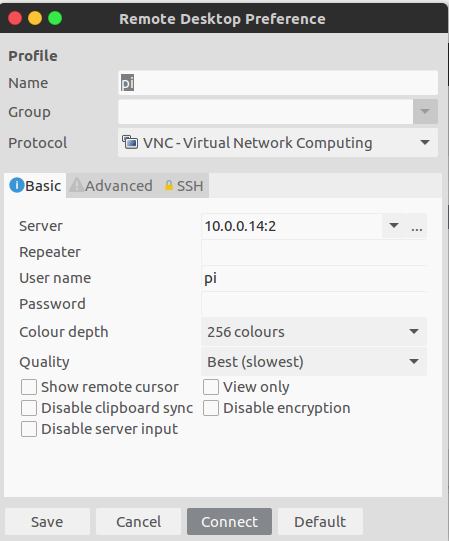
\includegraphics[scale=0.4]{raspberryremtoeconfig.png}
	\caption{Ubuntu远程连接配置}
	\label{fig:raspberryremtoeconfig}
\end{figure}

\subsection{Ubuntu远程Ubuntu}

这里的两台机器都是Ubuntu 16.04 LTS系统,xrdp支持不了13.10的GNOME了,解决办法是安装xfce界面。被远程的机器上安装必须的组件:

\begin{lstlisting}[language=Bash]
#安装xrdp
sudo apt-get install xrdp -y
#安装vnc4server
sudo apt-get install vnc4server tightvncserver -y
#安装xfce4
sudo apt-get install xubuntu-desktop -y
sudo /etc/init.d/xrdp restart
# 指定桌面管理器
echo "gnome-session --session=gnome-classic" > ~/.xsession
\end{lstlisting}

最后一个命令的作用是由于安装了gnome桌面,ubuntu16.04中同时存在unity、GNOME多个桌面管理器,需要启动的时候指定一个,不然即使远程登录验证成功以后,也只是背景。在Ubuntu上使用Remmina Remote Desktop Client即可链接远程桌面。

\subsection{Mac Book远程Fedora}

在Mac Book远程Linux主机选择的是XQuartz,安装好XQuartz后,直接在从XQuartz打开的终端中运行:

\begin{lstlisting}[language=Bash]
ssh -X dolphin@10.0.0.10
\end{lstlisting}

直接在命令行中启动图形化界面,会在Mac上显示Linux主机上的软件原生GUI界面,就像软件在本机运行一样。X11是X Window System主版本11的缩写,它不光是一个基本的GUI软件,X11也被定义为一个网络协议,因为X11提供了非常灵活的网络访问接口。SSH 的 X11 forwarding 特性可以使 X client 和 X server 安全地通讯。使用 X11 forwarding 后,从 X client 到 X Server 方向的数据先被送至 SSH server,SSH server 利用和 SSH client 的安全通道转发给 SSH client,再由 SSH client 转发给 X server,从 X server 到 X client 的数据流同理。这里 SSH server 和 SSH client 充当了 X client 和 X server 间数据的转发器,由于 SSH server 和 X client、SSH client 和 X server 一般在同一台机器上,它们之间是一种安全的进程间通讯,而 SSH server 和 SSH client 间的通讯也是安全的,所以 X client 和 X server 间的通讯就是安全的。X在Unix-like系统上几乎完全占据统治地位。但是仍然有人尝试提供替代品和更多的选择,过去曾经有 Sun Microsystems 的 NeWS ,但它遭到市场失败;还有 NeXT 的 Display PostScript ,它最终转变为苹果电脑的 Quartz for Mac OS X 。

\subsection{常见问题}

得到了Initialization Sequence Completed消息,但是ping失败了 -- 这通常是服务端或客户端上的防火墙过滤了TUN/TAP网络接口从而阻止了VPN网络的流量。  

\subsubsection{ssl3\_get\_server\_certificate:certificate verify failed}

在Mac中,连接好了并没有显示IP的变化。This computer's apparent public IP address was not different after connecting to client. It is still 45.76.205.201.This may mean that your VPN is not configured correctly.


\paragraph{OpenVPN is connected to the server but your IP address does not change}

If OpenVPN connects to the server properly but your IP address does not change, you are probably missing the "--redirect-gateway" option. Add the following line:
--redirect-gateway def1 to your configuration file.

By default, OpenVPN only sends some traffic through the VPN — traffic that is specifically destined for the VPN network itself. The "--redirect-gateway" option tells OpenVPN to send all traffic through the VPN. (Leave out the "--" when it is put in the configuration file.)

An alternative to putting "redirect gateway def1" in the configuration file is to "push" it from the VPN server to the client.

\section{Nmap(GNU General Public License)}

Nmap(Network Mapper),网络映射器,是一款开放源代码的网络探测和安全审核的工具。
它的设计目标是快速地扫描大型网络,当然用它扫描单个主机也没有问题。
Nmap以新颖的方式使用原始IP报文来发现网络上有哪些主机,
那些主机提供什么服务(应用程序名和版本),那些服务运行在什么操作系统(包括版本信息),
它们使用什么类型的报文过滤器/防火墙,以及一堆其它功能。虽然Nmap通常用于安全审核,
许多系统管理员和网络管理员也用它来做一些日常的工作,比如查看整个网络的信息,
管理服务升级计划,以及监视主机和服务的运行。
Nmap脚本引擎(Nmap Script Engine)是Nmap最有力灵活的的一个特性。
它允许用户撰写和分享一些简单的脚本来一些较大的网络进行扫描任务。
基本上这些脚本是用Lua编程语言来完成的。通常Nmap的脚本引擎可以完成很多事情。

\subsection{主机发现(Host Discovery)}

主机发现顾名思义就是发现所要扫描的主机是否是正在运行的状态。
输入如下命令开始主机扫描

\begin{lstlisting}[language=Bash]
nmap -F -sT -v nmap.org
# 主机发现,生成存活主机列表
nmap -sn -T4 -oG Discovery.gnmap 192.168.24.0/24
grep "Status: Up" Discovery.gnmap | cut -f 2 -d ' ' > LiveHosts.txt
\end{lstlisting}

\begin{itemize}
	\item{-F}扫描100个最有可能开放的端口,F表示快速模式(Fast Model),
	比默认模式扫描更少的端口(Scan fewer ports than the default scan),
	如果需要扫描更多的端口,指定p参数,如下命令行片段所示:
	
	\begin{lstlisting}[language=Bash]
	nmap -p 0-10000 -A -v <Host>
	\end{lstlisting}
	
	端口号最好分段指定,否则扫描的速度会非常缓慢,
	例如需要扫描0-65535端口,可以先扫描0-10000端口,
	再扫描10001-20000,依次类推。
	
	\item{-v}获取扫描的信息
	\item{-sT(Scan using TCP)}采用的是TCP扫描,不写也是可以的,默认采用的就是TCP扫描
	\item{-sn参数表示ping扫描,禁用端口扫描}
	\item{-oG表示输出Grepable格式}
\end{itemize}

Nmap输出的是扫描目标的列表,以及每个目标的补充信息,至于是哪些信息则依赖于所使用的选项。
“所感兴趣的端口表格”是其中的关键。那张表列出端口号,协议,服务名称和状态。
状态可能是 open(开放的),filtered(被过滤的), closed(关闭的),或者unfiltered(未被过滤的)。
Open(开放的)意味着目标机器上的应用程序正在该端口监听连接/报文。 
filtered(被过滤的) 意味着防火墙,过滤器或者其它网络障碍阻止了该端口被访问,
Nmap无法得知 它是 open(开放的) 还是 closed(关闭的)。 
closed(关闭的) 端口没有应用程序在它上面监听,但是他们随时可能开放。 
当端口对Nmap的探测做出响应,但是Nmap无法确定它们是关闭还是开放时,
这些端口就被认为是 unfiltered(未被过滤的) 如果Nmap报告状态组合 
open|filtered 和 closed|filtered时,那说明Nmap无法确定该端口处于两个状态中的哪一个状态。
当要求进行版本探测时,端口表也可以包含软件的版本信息。
当要求进行IP协议扫描时 (-sO),Nmap提供关于所支持的IP协议而不是正在监听的端口的信息。
获取远程主机的系统类型及开放端口:

\begin{lstlisting}[language=Bash]
nmap -sS -P0 -sV -O <target>
\end{lstlisting}

\subsection{端口扫描(Port Scanning)}

端口扫描是Nmap最基本最核心的功能,用于确定目标主机的TCP/UDP端口的开放情况。
端口扫描简单示例如下代码片段所示:

\begin{lstlisting}[language=Bash]
#服务扫描
nmap-T4 -sV targetip 

#扫描淘宝IP
nmap -p 0-1000 -v 218.201.46.124
nmap -T4 -A -v 218.201.46.124

# 扫描指定主机的3306端口
nmap -sS -p 3306 -v 192.168.31.25
\end{lstlisting}

通过扫描可以发现一些主机信息,比如淘宝的数字证书用的是GlobalSign,
加密位数是2048,签名算法是sha256WithRSAEncryption,
操作系统猜测是Linux系列的,内核版本可能是3.X或者2.6.X,
具体信息如下。

\begin{lstlisting}
443/tcp open  ssl/http Tengine httpd
|_http-server-header: Tengine
|_http-title: 501 Not Implemented
| ssl-cert: Subject: commonName=*.tmall.com/organizationName=Alibaba (China) Technology Co., Ltd./stateOrProvinceName=ZheJiang/countryName=CN
| Issuer: commonName=GlobalSign Organization Validation CA - SHA256 - G2/organizationName=GlobalSign nv-sa/countryName=BE
| Public Key type: rsa
| Public Key bits: 2048
| Signature Algorithm: sha256WithRSAEncryption
| Not valid before: 2015-12-14T10:38:38
| Not valid after:  2016-12-14T10:38:38
| MD5:   5d67 3ca3 7f0e 2ab7 7b4f 59d5 0700 7223
|_SHA-1: d048 e9cf 5487 5030 9f26 e638 7d3f 94ad a2b3 e6fa
\end{lstlisting}

默认情况下,Nmap会扫描1000个最有可能开放的TCP端口。

1)公认端口(0~1023),又称常用端口,为已经公认定义或为将要公认定义的软件保留的。
这些端口紧密绑定一些服务且明确表示了某种服务协议。如80端口表示HTTP协议。
2)注册端口(1024~49151),又称保留端口,这些端口松散绑定一些服务。
3)动态/私有端口(49152~65535)。理论上不应为服务器分配这些端口。
按协议类型可以将端口划分为TCP和UDP端口。
1)TCP端口是指传输控制协议端口,需要在客户端和服务器之间建立连接,
提供可靠的数据传输。如Telnet服务的23端口。
2)UDP端口是指用户数据包协议端口,不需要在客户端和服务器之间建立连接。
常见的端口有DNS服务的53端口。
有的服务器为了安全会修改默认端口,
比如将ssh默认的22端口修改为50000,
不过通过Nmap扫描也会很容易的发现。
详细的扫描指令如下所示:

\begin{lstlisting}[language=Bash]
nmap -sS -sU -T4 -A -v -PE -PP -PS80,443 -PA3389 -PU40125 -PY -g 53 --script "default or (discovery and safe)" 12.26.32.14 
\end{lstlisting}

\begin{itemize}
	\item{-sS参数(TCP SYN Scan)可以利用基本的SYN扫描方式探测其端口开放状态}
	\item{-sU参数代表UDP Scan}
	\item{-T<0-5>: Set timing template (higher is faster)}
	\item{-A: Enable OS detection, version detection, script scanning, and traceroute}
	\item{-v: Increase verbosity level (use -vv or more for greater effect)}
	\item{-PE/PP/PM: ICMP echo, timestamp, and netmask request discovery probes}
	\item{-PS/PA/PU/PY[portlist]: TCP SYN/ACK, UDP or SCTP discovery to given ports}
	\item{-g/--source-port <portnum>: Use given port number}
\end{itemize}


\paragraph{"ppp0" is not an ethernet device}在使用nmap扫描时候,提示 

\begin{lstlisting}
Only ethernet devices can be used for raw scans on Windows, and "ppp0" is not an ethernet device. Use the --unprivileged option for this scan. QUITTING!
\end{lstlisting}

因为用Nmap扫描时,不能用pppoe的拨号口,只能用以太网口。
根据提示带参数--unprivileged就可以了,注意扫描的命令不能带-A参数,
否则会要求root权限,无法启动扫描。 


\subsection{版本侦测(Version Detection)}

版本侦测在后面添加sV(Service/Version)参数即可。

\begin{lstlisting}[language=Bash]
-sV: Probe open ports to determine service/version info
\end{lstlisting}

\subsection{Zenmap}

Zenmap是Nmap的官方GUI,可以运行在Linux, Windows, Mac OS X, BSD等操作系统上。

\begin{lstlisting}[language=Bash]
# Mac下获取Zenmap安装文件
wget -c https://nmap.org/dist/nmap-7.31.dmg
\end{lstlisting}


\section{tmux}

tmux是一个优秀的终端复用软件,类似GNU Screen,但来自于OpenBSD,采用BSD授权。使用tmux的好处之一就是可以保存会话,避免网络不稳定带来的影响。

\begin{tabular}{|c|p{8cm}|c|}
	\hline
	\multirow{1}{*}{键}
	& \multicolumn{1}{c|}{作用}  \\			
	\cline{1-2}
	Ctrl + b d  & 返回主 shell ,detach, tmux 依旧在后台运行,里面的命令也保持运行状态\\
	\hline
	C-b ? & 显示快捷键帮助\\
	\hline
\end{tabular}


\section{Raspberry Pi}

\subsection{Raspberry Pi远程}

安装步骤:

\begin{lstlisting}[language=Bash]
# 安装tightvncserver
sudo apt-get install tightvncserver -y
# 设置密码
vncpasswd
\end{lstlisting}

\section{Widgets}

\subsection{autojump}

autojump可以让你一键跳转到目标目录,一般情况下,很难准确的记忆清楚目标目录的准确路径,特别是目录嵌套比较深的时候。不停的重复使用cd命令一级或多级跳转显得有点笨拙。此时就可以使用autojump命令,只需要输入路径的关键字即可,比如只记得路径中隐约包含有关键字“jiangxiaoqiang”,那么仅仅输入命令autojump jiang,就可以自动跳转到对应的路径下。安装autojump:

\begin{lstlisting}[language=Bash]
sudo apt-get install autojump -y
# 给autojump命令设置别名
alias j='autojump'
# 从源代码安装autojump
git clone git://github.com/joelthelion/autojump.git
chmod 755 install.py
./install.py

# 将当前路径添加到autojump的搜索库
autojump -a 'pwd'
\end{lstlisting}

为了进一步简化目录跳转命令,可以直接添加命令autojump的别名:

\begin{lstlisting}[language=Bash]
alias j='autojump'
\end{lstlisting}

有时会出现如下的提示:Please source the correct autojump file in your shell's startup file. For more information, please reinstall autojump and read the post installation instructions.为了暂时激活autojump应用,即直到你关闭当前会话或打开一个新的会话之前让autojump均有效,需要以常规用户身份运行下面的命令:

\begin{lstlisting}[language=Bash]
# 在Linux系统下
source /usr/share/autojump/autojump.sh on startup
# 在Mac OS X下
source ~/.autojump/etc/profile.d/autojump.sh
# 也可运行如下命令
[[ -s /Users/dolphin/.autojump/etc/profile.d/autojump.sh ]] && source /Users/dolphin/.autojump/etc/profile.d/autojump.sh
\end{lstlisting}

为了使得autojump在BASH shell中永久有效,需要运行下面的命令。

\begin{lstlisting}[language=Bash]
echo '. /usr/share/autojump/autojump.sh'>>~/.bashrc
# 在Mac OS X下
echo '. ~/.autojump/etc/profile.d/autojump.sh'>>~/.bashrc
\end{lstlisting}

\section{Git}

\subsection{配置}

\subsection{常见问题}


\paragraph{error setting certificate verify location}

当你通过HTTPS访问Git远程仓库,如果服务器的SSL证书未经过第三方机构签署,那么Git就会报错。这是十分合理的设计,毕竟未知的没有签署过的证书意味着很大安全风险。但是,如果你正好在架设Git服务器,而正式的SSL证书没有签发下来,你为了赶时间生成了自签署的临时证书。

\begin{lstlisting}[language=Bash]
env GIT_SSL_NO_VERIFY=true git clone https://<host_name/git/project.git
\end{lstlisting}

或者将Git设置为不允许ssl认证:


\begin{lstlisting}[language=Bash]
git config --system http.sslverify false
\end{lstlisting}


\section{ssh}

\subsection{免密登陆}

免密登录需要注意的是,.ssh文件夹下的authorize\_key文件的权限需要是600。

\begin{lstlisting}[language=Bash]
ssh -p 22 pi@192.168.31.25 'mkdir -p .ssh && cat >> .ssh/authorized_keys' < ~/.ssh/id_rsa.pub
\end{lstlisting}

\subsection{Session时间}

在使用ssh的过程中,经常会遇到一会儿没有操作就自动断开了,不是非常方便。

\paragraph{ClientAliveInterval}

修改/etc/ssh/sshd\_config配置文件 ClientAliveInterval 300(默认为0),参数的是意思是每5分钟,服务器向客户端发一个消息,用于保持连接,使用service sshd reload 让其修改后生效。如果发现还是有问题,可以试着把300设置小一点,例如60。

\paragraph{ClientAliveCountMax}

另外,至于ClientAliveCountMax, 使用默认值3即可.ClientAliveCountMax表示服务器发出请求后客户端没有响应的次数达到一定值, 就自动断开。

\paragraph{ControlPersist 4h}

在./ssh/config中添加一行:

\begin{lstlisting}[language=Bash]
ControlPersist 4h
\end{lstlisting}

When used in conjunction with ControlMaster, specifies that the master connection should remain open in the background (waiting for future client connections) after the initial client connection has been closed. If set to no, then the master connection will not be placed into the background, and will close as soon as the initial client connection is closed. If set to yes or 0, then the master connection will remain in the background indefinitely (until killed or closed via a mechanism such as the “ssh -O exit”). If set to a time in seconds, or a time in any of the formats documented in sshd\_config, then the backgrounded master connection will automatically terminate after it has remained idle (with no client connections) for the specified time\footnote{\url{http://man.openbsd.org/ssh_config.5}}.现在你每次通过SSH与服务器建立连接之后,这条连接将被保持4个小时,即使在你退出服务器之后,这条连接依然可以重用,因此,在你下一次(4小时之内)登录服务器时,你会发现连接以闪电般的速度建立完成,这个选项对于通过scp拷贝多个文件提速尤其明显,因为你不在需要为每个文件做单独的认证了。

\subsection{代理转发}

\paragraph{本地转发Local Forward}将本地机(客户机)的某个端口转发到远端指定机器的指定端口. 工作原理是这样的, 本地机器上分配了一个 socket 侦听 port 端口, 一旦这个端口上有了连接, 该连接就经过安全通道转发出去, 同时远程主机和 host 的 hostport 端口建立连接. 可以在配置文件中指定端口的转发. 只有 root 才能转发特权端口. 

\paragraph{远程转发Remote Forward}

\subsection{rsync}

在使用scp命令时,无法实现断点续传。rsync是类unix系统下的数据镜像备份工具——remote sync。一款快速增量备份工具 Remote Sync,远程同步 支持本地复制,或者与其他SSH、rsync主机同步。

\section{Curl}

内部接口测试:

\begin{lstlisting}[language=Bash]

\end{lstlisting}

外部接口测试:


\begin{lstlisting}[language=Bash]

\end{lstlisting}

\section{Git}

\subsection{merge}

配置Meld为默认合并工具:

\begin{lstlisting}[language=Bash]
git config --global merge.tool meld
\end{lstlisting}

\section{Google Chrome}

\subsection{Source Map}

截止目前几乎没有浏览器完全原生支持es6标准,对于这种情况,Chrome引入了source-map文件,标识es5代码对应的转码前的es6代码哪一行,唯一要做的就是配置webpack自动生成source-map文件,这也很简单,在webpack.config.js中增加一行配置即可(需要重新启动webpack-dev-server使配置生效)

\subsection{Replay XHR}

有时在开发时,可以直接在Network中点击右键,在菜单中重复发送XHR请求(Replay XHR),不需要再次进入界面模拟请求,可以提交不少效率。

\subsection{Google Chrome SSH}

\section{Zentao}

\subsection{常见问题}

运行禅道需要PHP环境,在Ubuntu 16.04上面安装PHP:

\begin{lstlisting}[language=Bash]
sudo apt-get install php7.0 -y
\end{lstlisting}

由于80端口已经被占用,修改禅道的默认端口,在文件文件中。

\begin{lstlisting}
/opt/zbox/etc/apache/http.conf
\end{lstlisting}

由于以前电脑有安装MySQL,所以3306端口被占用了。所以在启动禅道是会提示MySQL端口已经被占用,执行如下命令修改禅道的MySQL端口即可:

\begin{lstlisting}[language=Bash]
/opt/zbox/zbox -mp 3307
\end{lstlisting}

\section{LaTex}

\subsection{安装}

\begin{lstlisting}[language=Bash]
# Ubuntu下安装Texlive
sudo apt-get install texlive -y
\end{lstlisting}

\subsection{字体}

Computer Modern是自由软件TeX的默认字体,为美国计算机科学家高德纳(Donald Knuth)使用METAFONT软件创造。但是此字体不是很漂亮,所以考虑换一个字体 。

\subsection{版面}

\paragraph{换行}Latex的自动拆单词换行是依靠字典的。如果遇到\LaTeX{}不认识的单词,他就不会换行了。后面的内容就会溢出。

\part{DB}

\section{Redis}

\subsection{安装}

这里是在Raspberry Pi上安装Redis:

\begin{lstlisting}[language=Bash]
# 下载源码
wget -c http://download.redis.io/releases/redis-3.2.9.tar.gz
# 编译安装
make
make test
\end{lstlisting}


\section{MySQL}

\subsection{基础}

启动MySQL:

\begin{lstlisting}[language=Bash]
mysqld

# Mac中启动MySQL,同理停止的参数为stop,重启的参数为restart
sudo /usr/local/MySQL/support-files/mysql.server start

# 防火墙添加端口
sudo iptables -A INPUT -p tcp --dport 3306 -j ACCEPT /*允许包从3306端口进入*/
sudo iptables -A OUTPUT -p tcp --sport 3306 -m state --state ESTABLISHED -j ACCEPT /*允许从3306端口进入的包返回*/

# 查看iptables
sudo iptables --list
SHOW DATABASES                                //列出 MySQL Server 数据库。
SHOW TABLES [FROM db_name]                    //列出数据库数据表。
SHOW TABLE STATUS [FROM db_name]              //列出数据表及表状态信息。
SHOW COLUMNS FROM tbl_name [FROM db_name]     //列出资料表字段
SHOW FIELDS FROM tbl_name [FROM db_name],DESCRIBE tbl_name [col_name]。
SHOW FULL COLUMNS FROM tbl_name [FROM db_name]//列出字段及详情
SHOW FULL FIELDS FROM tbl_name [FROM db_name] //列出字段完整属性
SHOW INDEX FROM tbl_name [FROM db_name]       //列出表索引。
SHOW STATUS                                  //列出 DB Server 状态。
SHOW VARIABLES                               //列出 MySQL 系统环境变量。
SHOW PROCESSLIST                             //列出执行命令。
SHOW GRANTS FOR user                         //列出某用户权限
GRANT ALL PRIVILEGES ON *.* TO 'root'@'192.168.31.25'IDENTIFIED BY 'dolphin' WITH GRANT OPTION;
\end{lstlisting}

在使用MySQL会出现中文乱码问题,MySQL的字符集支持(Character Set Support)有两个方面:字符集(Character set)和排序方式(Collation)。对于字符集的支持细化到四个层次: 服务器(server),数据库(database),数据表(table)和连接(connection)。在Mac中,在etc目录下新建my.cnf文件,指定数据库编码:

\begin{lstlisting}[language=Bash]
[mysqld]
character-set-server=utf8
init_connect='SET NAMES utf8'
[mysql]
default-character-set=utf8
\end{lstlisting}

修改后,重新启动数据库。但是以前新建的表有可能还是采用的原来的编码,使用如下语句进行修改:

\begin{lstlisting}[language=SQL]
--检查数据表所有字段的状态	
show full columns from book; 
--发现address字段的Collation项非utf8,改成utf8
alter table book change publisher publisher varchar(512) character set utf8 collate utf8_unicode_ci not null;
\end{lstlisting}


\subsection{MySQL远程连接}

本来以为安装完毕MySQL就可以自动进行远程连接,结果竟然花了半天时间才搞定。安装完毕后MySQL默认是不能远程连接的,由于在其他主机上用nmap无法扫描到端口3306,开始还以为是防火墙的缘故,在错误的道路上研究了许久,最后竟然在本机也无法扫描到端口。才明白MySQL是与localhost绑定而不是与IP绑定。在目录/etc/mysql/目录中修改配置文件my.cnf:

\begin{lstlisting}[language=Bash]
# Instead of skip-networking the default is now to listen only on
# localhost which is more compatible and is not less secure.
bind-address            = 192.168.31.25
\end{lstlisting}

默认是127.0.0.1,是一个回环地址,只有本机请求本机,目标地址才会是127.0.0.1,此时需要在其他主机请求,需要将绑定IP改为网卡地址, 也就是外网IP, 因为远程连接数据库目标IP肯定是公网IP. 不过还可以改成0.0.0.0,这样就表示监听所有IP, 只要端口一样, 网卡都会把请求传给进程。如果不在配置文件中修改地址,则需要在启动时指定绑定地址:

\begin{lstlisting}[language=Bash]
sudo mysqld --bind-address=192.168.31.25
\end{lstlisting}

绑定好地址后,使用命令sudo lsof:3306查看。如果填写的绑定地址是192开头,那么最终只有192开头的局域网里的机器能够远程连接MySQL,有时一台设备可能会处于多个局域网中,那么此时另一个局域网的设备就无法远程连接MySQL了。此时可以将绑定地址修改为0.0.0.0,即允许所有的IP连接到MySQL,相应的MySQL的安全性相应的就降低了。

\subsection{Mac中MySQL初始密码}

step1:

苹果->系统偏好设置->最下边点mysql 在弹出页面中 关闭mysql服务(点击stop mysql server)

step2:

进入终端输入:cd /usr/local/mysql/bin/
回车后 登录管理员权限 sudo su
回车后输入以下命令来禁止mysql验证功能 ./mysqld\_safe --skip-grant-tables \&
回车后mysql会自动重启(偏好设置中mysql的状态会变成running)

step3. 
输入命令 ./mysql
回车后,输入命令 FLUSH PRIVILEGES; 
回车后,输入命令 SET PASSWORD FOR 'root'@'localhost' = PASSWORD('你的新密码');

\subsection{备份}

netstat -ln | grep mysql

mysqldump --sock=/var/run/mysqld/mysqld.sock -u root -p dolphin>dolphin.sql

\subsection{存储过程}

\begin{lstlisting}[language=SQL]
DELIMITER $$

CREATE DEFINER=`root`@`%` PROCEDURE `insert_initial_id`()
BEGIN  

DECLARE i INT DEFAULT 1;# can not be 0  
DECLARE j INT DEFAULT 10000000;# can not be 0  


WHILE i<99999999 && j < 10000050
DO  
	insert into douban_book_id(isscapy,douban_book_id) values (0,j);  
	SET i=i+1;  
	set j=j+1;
END WHILE ;  
commit;  

END$$
DELIMITER ;
\end{lstlisting}


\subsection{mycli}

MyCli 是一个 MySQL 命令行工具,支持自动补全和语法高亮。也可用于 MariaDB 和 Percona。安装mycli:

\begin{lstlisting}[language=Bash]
pip install mycli
brew install mycli
\end{lstlisting}

在Ubuntu下远程配置如图\label{raspberryremtoeconfig}所示:

\subsection{常见问题}

\paragraph{ERROR 2002 (HY000): Can't connect to local MySQL server through socket '/tmp/mysql.sock'}

mysql使用unix socket或者tcp来连接数据库进行通讯,默认不加 -h选项时使用的就是localhost即unixsocket,此时会通过/tmp/mysql.sock来通讯,但是在配置文件中默认生成的socket文件是在/var/lib/mysql/mysql.sock(不同安装可能不同,建议查看/etc/my.cnf确认),所以要想mysql使用这个文件通讯,最简单的方法就是建立软链接,一劳永逸,此为方法一

方法二就是强制mysql使用tcp通讯,因为127.0.0.1对于mysql来说走的是tcp协议而非unixsocket,这种方法的弊端就是每次都要指明本地地址127.0.0.1

\part{Network}

\section{PAC}

\subsection{PAC简介}

PAC是proxy auto-config的缩写。PAC文件是纯文本格式的,实际上就是JavaScript文件。PAC最简单的格式就是包含一个叫FindProxyForURL的JavaScript函数,IE通过传入两个变量来调用这个函数。一个是用户流量的地址的URL全路径,一个是这个URL中的主机名host。在日常生活中浏览器中设置代理很简单,但是当你来回切换时总是觉得很烦,你可以使用pac脚本自动判断是否走代理,方便省去了来回手动切换的烦恼。

\subsection{PAC实例}

一个最简单的PAC脚本:

\begin{lstlisting}[language=VBScript]
function FindProxyForURL(url,host){
	return "DIRECT";
}
\end{lstlisting}

参数url是用户输入的url,参数host是url中的主机名。PAC文件返回值有三种类型:

\begin{itemize}
	\item{DIRECT直连不通过代理}
	\item{PROXY www.lybbn.cn:8080 http通过8080端口代理上网,也可以使用ip:port的形式}
	\item{SOCKS5 www.lybbn.cn:8080 socks通过8080端口代理上网,可以使用ip:port形式}
\end{itemize}

\begin{lstlisting}[language=VBScript]
var FindProxyForURL = function(init, profiles) {
	return function(url, host) {
		"use strict";
		var result = init, scheme = url.substr(0, url.indexOf(":"));
		do {
			result = profiles[result];
			if (typeof result === "function") result = result(url, host, scheme);
		} while (typeof result !== "string" || result.charCodeAt(0) === 43);
		return result;
	};
}("+dolphin2", {
	"+dolphin2": function(url, host, scheme) {
		"use strict";
		if (/^59\.214\.215\.6$/.test(host)) return "+dolphin-proxy";
		if (/^10\.10\.1\.11$/.test(host)) return "+dolphin-proxy";
		return "DIRECT";
	},
	"+dolphin-proxy": function(url, host, scheme) {
		"use strict";
		if (/^127\.0\.0\.1$/.test(host) || /^::1$/.test(host) || /^localhost$/.test(host)) return "DIRECT";
		return "PROXY 10.55.10.2:8888";
	}
});
\end{lstlisting}

以上脚本说明,当IP为59.214.215.6或10.10.1.11时,使用代理dolphin-proxy,而代理dolphin-proxy设置的是代理机器的相关信息,代理机器的IP为10.55.10.2,代理的端口是8888。

\part{Engneering}

\section{通用规范}

\subsection{版本管理}

在项目的开发过程中,要求有明确的版本号,以前只是在正式发布版本的时候才会生成带版本号的文件,目前测试需要每次发布版本修改时定义版本号,方便测试进行问题识别。以前直接使用脚本生成的带有年月日的版本标志,但是还是需要进一步规范化。由于发布采用的自动化脚本,在启动程序时需要指定明确的文件名称,文件名称与版本号有关联,所以考虑将版本号保存到一个文件里面,使用Gradle构建程序和发布程序时都读取此文件中的版本号。Given a version number MAJOR.MINOR.PATCH, increment the:

\begin{itemize}
	\item{MAJOR version when you make incompatible API changes,}
    \item{MINOR version when you add functionality in a backwards-compatible manner}
	\item{PATCH version when you make backwards-compatible bug fixes.}
\end{itemize}

Additional labels for pre-release and build metadata are available as extensions to the MAJOR.MINOR.PATCH format.在项目的根目录下新建version.properties文件,文件中定义版本号:

\begin{lstlisting}
VERSION_CODE=1.0.2
\end{lstlisting}

在Gradle中读取版本号:

\begin{lstlisting}
version = getVersionCode()

def getVersionCode() {
	def versionFile = file('/Users/dolphin/source/credit-system/gradle/version.properties')
	if (versionFile.canRead()) {
		def Properties versionProps = new Properties()
		versionProps.load(new FileInputStream(versionFile))
		def versionCode = versionProps['VERSION_CODE'].toString()
		/*def runTasks = gradle.startParameter.taskNames        //仅在assembleRelease任务是增加版本号
		if ('assembleRelease' in runTasks) {
			versionProps['VERSION_CODE'] = (++versionCode).toString()
			versionProps.store(versionFile.newWriter(), null)
		}*/
		return versionCode
	} else {
		throw new GradleException("Could not find version.properties!")
	}
}
\end{lstlisting}

此处文件路径写的是绝对路径,如果仅仅在本机进行构建问题不大,但是一般都是团队协作,所以写成相对路径会比较妥当。可以写成如下:

\begin{lstlisting}
File versionFile = file("$rootDir/cc-web-boot/src/main/resource/version.properties")
\end{lstlisting}

其中\$rootDir表示项目的根目录,比如有一个叫做dolphin的项目,那么rootDir就是dolphin目录,另外还有一个projectDir的变量和buildDir的变量。projectDir就是dolphin/src目录,buildDir就是dolphin/src/build目录。如果是多个Project组成的项目,那么projectDir就是rootDir/projectName,buildDir就是dolphin/projectName/build。




\end{document}
\theend
